\documentclass[12pt]{article}
\usepackage{mathtools}
\usepackage{graphicx}
\usepackage{amsmath}
\usepackage{amsfonts}
\usepackage{microtype}
\usepackage{hyperref}
\usepackage{tikz-cd}
\usepackage{amssymb}
\usepackage{comment}
\usepackage{mymacros}
\usepackage{caption}
\usepackage{subcaption}
\usepackage{biblatex}
\usepackage{float}
\usepackage{geometry}
\usepackage{hyperref}
 \geometry{
 a4paper,
 total={170mm,257mm},
 left=25mm,
 top=20mm,
 }
 
\renewenvironment{abstract}
{\small
 \begin{center}
 \bfseries \abstractname\vspace{-.5em}\vspace{0pt}
 \end{center}
 \list{}{
   \setlength{\leftmargin}{2cm}%
   \setlength{\rightmargin}{\leftmargin}%
 }%
 \item\relax}
{\endlist}




\addbibresource{refrences.bib}

\setlength{\parindent}{0cm} 
\setlength{\parskip}{1em}

\graphicspath{{./img/}}

\begin{document}
\begin{center}
  \Large \textbf{Solving the 1D-Poisson Equation Numerically}

  \large\text{Kristian Gjestad Vangsnes}
  
  \textit{Department of physics, University of Oslo}


  \text{Date: 9. September 2019}

  Github repository: \cite{kristian}
\end{center}
\begin{abstract}
  I study three algorithms solving the one-dimentional Poisson equation with a source term, which is done by converting the problem into a linear algebra problem. I compare the efficiency and precision of the algorithms and find that an optimized algorithm perform almost five times as fast as a general algorithm. Solving the problem using LU decomposition was found to be the least effective. In addition I found that the loss of precision becomes apparent when the number of gridpoints exceeds $1,2\times 10^5$.


\end{abstract}
\section{Introduction}
In this project I will study numerical algorithms which solves Poisson's equation in one dimension which is a first order differential equation. This is the equation which describes the change of an electric potential. Two algorithms will be based on Gaussian-elimination and is programmed on a lower level using c++, while the third algorithm is the famous LU-decomposition and will be computed using the linear algebra library Armadillo.

The focus of this report is to compare the efficiency and precision of the algorithms. I will first compare the numerical solution with the exact solution for the problem. Then I want to compare the times of a general algorithm, an algorithm specialized for the problem and the LU decomposition. Then I will look at the relative error of an algorithm and search for when the loss of precision becomes apparent.

\section{Theory}
The one-dimentional Poisson equation 
with Dirichlet boundary conditions reads 

\begin{equation*}
 -u''(x)=f(x),\quad x\in (0,1),\quad u(0)=u(1)=0.
\end{equation*}

I will use the source term $f(x)=100e^{-10x}$. This gives the particular solution 
$u(x)=1-(1-e^{-10})x-e^{-10x}$. I will compare the numerical solution to this exact solution.

I will also compute the relative error for the algorithms in order to see how accurate they are. The relative error is defined as 
$$ \epsilon=\log{\left|\frac{u_{numerical}-u_{exact}}{u_{exact}}\right|}.$$

\section{Numerical methods}
In order to model the equation in a computer I need to
discretize the solution, i.e.  $ u(x) \rightarrow v_i=v(x_i) $ where
 $x_i=x_0+ih=ih$ since $x_0=0$. I let $x_{n+1}=1$, this means $h=\frac{1}{n+1}$.
 From Taylor expanding $u(x\pm h)$ I get 
 $$u(x\pm h)=u(x)\pm hu'(x)+\frac{h^2}{2!}u''(x)\pm O(h^3)$$
I see that $u''(x)=\frac{u(x+h)+u(x-h)-2u(x)}{h^2}-O(h^4)$. Hence for the approximated solution
 I get that $$-\frac{v_{i+1}+v_{i-1}-2v_i}{h^2}=f_i\quad \text{for i}=1,...,n$$ where $f_i=f(x_i)$. 
 If I set $g_i=h^2f_i$ I get that $2v_i-v_{i+1}-v_{i-1}=g_i$. 
 This is just $n$ equations, given by $i=1,...,n$. I can write this in matrix form as
 $$\mathbf{A}\mathbf{v}=\mathbf{g}, $$ where $\mathbf{A}$ is a $n\times n$ 
 tridiagonal matrix on the form 
 \begin{equation}
   \label{eq:matrix}
  \mathbf{A}=\begin{bmatrix}
    2 & -1 & 0 & \dots & ... & 0 \\
    -1 & 2 & -1 & 0 & ... & 0 \\
    0  & -1 & 2 & -1 & 0 & ... \\
    \vdots & 0 & \ddots & \ddots & \ddots & ...\\
    0 & ... & ... & -1 & 2 & -1\\
    0 & ... & ... & 0 & -1 & 2 
  \end{bmatrix}
\end{equation}

 $\mathbf{v}$ and $\mathbf{g}$ are vectors on the form 
 $$\mathbf{v}=\begin{bmatrix}
   v_1\\v_2\\\vdots\\v_n
 \end{bmatrix}
 \qquad
 \mathbf{g}=\begin{bmatrix}
   g_1\\g_2\\\vdots\\g_n
 \end{bmatrix}
 $$

 The relative error is computed by 
 \begin{equation}\label{eq:rel_error}
  \epsilon=\log{\left|\frac{v_{i}-u_{i}}{u_{i}}\right|}
 \end{equation} 

 The error for the double derivative is approximated to be the next part of the Taylor expansion, meaning that $\epsilon_{approx}\approx \frac{|u_0^{(4)}|}{12}h^2 $, as done in the lecture notes \cite{morten}[p.59]. 

 I also have to take into account the machine error which comes into play when I subtract two nearly equal numbers. If $(u_{\pm h}-u_0)$ is nearly zero, then I have $(u_{\pm h}-u_0)\approx \epsilon_M$, where $\epsilon_M$ is the machine error, which is less or equal $10^{-15}$ for double precision. Hence $|u_0''|=\left|\frac{(u_h+u_{-h}-2u_0)}{h^2} \right|=\left|\frac{((u_h-u_0)+(u_{-h}-u_0)}{h^2} \right|\leq \frac{2\epsilon_M}{h^2}\approx \frac{2\times 10^{-15}}{h^2}$. The total error becomes 
 
 \begin{equation}
  \label{eq:total_error}
  \epsilon_{tot}\leq \frac{2\times 10^{-15}}{h^2}+\frac{|u_0^{(4)}|}{12}h^2\approx 2n^2\times 10^{-15}+\frac{|u_0^{4}|}{12n}
 \end{equation}. 

 I can take the derivative of $\epsilon_{tot}$, set it equal to zero and using that $u''(x)=-f(x)$ to find the where the error is smallest. When I do this I find that the number of gridpoints to minimize the error is given by
 
 \begin{equation}
   \label{eq:error_n}
  n=\left(\frac{|u_0^{(4)} |}{24}\times 10^{15}\right)^{-\frac{1}{4}}
\end{equation}

If $n>\left(\frac{|u_0^{(4)} |}{24}\times 10^{15}\right)^{-\frac{1}{4}}$ the round off errors will become apparent and dominating.

 \subsection{General algorithm}
 The general algorithm to solve a set of equation on a tridiagonal form is done by Gaussian elimination, and is called the Thomas algorithm \cite{thomas}.  On matrix form the problem is $\mathbf{A}\mathbf{v}=\mathbf{g}$. Where $\mathbf{v}$ contains the unknowns $v_i$. In this case the unknowns are the solution to the Poisson equation at $x_i=ih$, i.e. $v(x_i)=v_i$.
 $$
 \mathbf{A}=  \begin{bmatrix}
  d_1 & b_1 & 0 & \dots & ... & 0 \\
  a_1 &d_2 & b_2 & 0 & ... & 0 \\
  0  & a_2 & d_3 & b_3 & 0 & ... \\
  \vdots & 0 & \ddots & \ddots & \ddots & ...\\
  0 & ... & ... & a_{n-2} & d_{n-1} & b_{n-1}\\
  0 & ... & ... & 0 & a_{n-1} & d_{n} 
 \end{bmatrix}, \qquad \mathbf{g}=\begin{bmatrix}
  g_1 \\ g_2 \\ \vdots \\ g_n
 \end{bmatrix}.
 $$
I see that the two first equations are 
\begin{equation}
  d_1v_1+b_1v_2=g_1
  \label{eq:eq1}
\end{equation}
\begin{equation}
  a_1v_1+d_2v_2+b_2d_3=g_2
  \label{eq:eq2}
\end{equation}

I see that if I multiply eq (\ref{eq:eq1}) by $\frac{a_1}{d_1}$ and subtract it from eq(\ref{eq:eq2}) I see that eq(\ref{eq:eq2}) becomes $$ (d_2-\frac{a_1b_1}{d_1})=g_2-\frac{a_1g_1}{d_1}. $$

This is called forward substitution and for a tridiagonal matrix the general formula for the new elements is given by
$$\tilde{d}_{i+1}=d_{i+1}-\frac{a_ib_i}{\tilde{d_i}}$$  $$\tilde{g}_{i+1}=g_{i+1}-\frac{a_i\tilde{g_i}}{\tilde{d_i}}$$ Where $\tilde{d_1}=d_1$ and $\tilde{g}_1=g_1$. Now the problem is on the form $\mathbf{\tilde{A}}\mathbf{v}=\mathbf{\tilde{g}}$ where $$
\mathbf{\tilde{A}}=  \begin{bmatrix}
 \tilde{d}_1 & b_1 & 0 & \dots & ... & 0 \\
 0 &\tilde{d}_2 & b_2 & 0 & ... & 0 \\
 0  & 0 & \tilde{d}_3 & b_3 & 0 & ... \\
 \vdots & 0 & \ddots & \ddots & \ddots & ...\\
 0 & ... & ... & 0 & \tilde{d}_{n-1} & b_{n-1}\\
 0 & ... & ... & 0 & 0 & \tilde{d}_{n} 
\end{bmatrix}, \qquad \mathbf{g}=\begin{bmatrix}
 \tilde{g}_1 \\ \tilde{g}_2 \\ \vdots \\ \tilde{g}_n
\end{bmatrix}.
$$
To get the problem to a diagonal form I have to perform a backward substitution, this is done component wise by 
$$v_{n-i}=\frac{\tilde{g}_{n-i}-b_{n-i}v_{n+1-i}}{\tilde{d}_{n-i}}$$ where $v_{n}=\frac{\tilde{g}_n}{\tilde{d}_n}$. 

When I start to count from 0 to $n-1$ (as in c++) the algorithm goes as follows:

\begin{center}
  \begin{tabular}{||c||}
    \hline\hline
    \textbf{General Algorithm}\\
    \hline\hline
    Forward substitution \\
    \textbf{for} $i=0,1,2,...,n-1$\\
      $d_{i+1}-=a_ib_i/d_i$ \\
      $g_{i+1}-=a_ig_i/d_i$ \\
      \textbf{End loop} \\
      Backward substitution \\
      $v_{n-1}=g_{n-1}/d_{n-1}$\\
      \textbf{for i=2, 3, ..., n} \\
      $v_{n-i}=(g_{n-i}-b_{n-i}v_{n+1-i})/d_{n-i}$\\ 
      \textbf{End loop}\\
      \hline\hline
  \end{tabular}
\end{center}
The number of floating points operations (FLOPS) performed in this general algorithm is $9n$, $6n$ FLOPS in the forward substitution, $2n$ subtractions, $2n$ multiplications and $2n$ divisions. $3n$ FLOPS in the backward substitution, $n$ subtraction, $n$ multiplication and $n$ division.


\subsection{Specialized algorithm}
When all the diagonal elements are equal and the off diagonal elements are equal I can make the algorithm more efficient. If I use the matrix for the Poisson equation given by (\ref{eq:matrix}), I get an even more specialized algorithm. For equal diagonal elements and equal off diagonal elements I get the following algorithm.


\begin{center}
  \begin{tabular}{||c||}
    \hline\hline
    \textbf{Specialized Algorithm for equal diagonal and off diagonal terms}\\
    \hline\hline
    Diagonal term is $d$ and off diagonal term is $a$.\\
    $d_0=d$\\
    Let $A=a^2$, I precalculate in order to save time.\\
    Forward substitution \\
    \textbf{for} $i=0,1,2,...,n-1$\\
      $d_{i+1}-=A/d_i$ Note \\
      $g_{i+1}-=a\times g_i/d_i$ \\
      \textbf{End loop} \\
      $v_{n-1}=g_{n-1}/d_{n-1}$\\
      Backward substitution \\
      \textbf{for i=2, 3, ..., n} \\
      $v_{n-i}=(g_{n-i}-a\times v_{n+1-i})/d_{n-i}$\\ 
      \textbf{End loop}\\
      \hline\hline
  \end{tabular}
\end{center}

This algorithm does $8n$ FLOPS, it does $5n$ FLOPS in the forward substitution, $2n$ subtractions, $2n$ divisions and $n$ multiplications. In the backward substitution I have $3n$ FLOPS, $n$ subtractions, $n$ multiplications and $n$ divisions.

As mentioned I can make an even better algorithm if the diagonal elements are $2$ and the off diagonal elements are $-1$. I can then use the following algorithm.

\begin{center}
  \begin{tabular}{||c||}
    \hline\hline
    \textbf{Specialized Algorithm for the Poisson problem}\\
    \hline\hline Note tha
    t the diagonal elemets are precalculated\\
    Forward substitution \\
    \textbf{for} $i=0,1,2,...,n-1$\\
      $g_{i+1}+=g_i/d_i$\\
      \textbf{End loop} \\
      Backward substitution \\
      $v_{n-1}=g_{n-1}/d_{n-1}$\\
      \textbf{for i=2, 3, ..., n} \\
      $v_{n-i}=(g_{n-i}+v_{n+1-i})/d_{n-i}$\\ 
      \textbf{End loop}\\
      \hline\hline
  \end{tabular}
\end{center}
 I see that since I have precalculated the diagonal elements and used that the off diagonal element is -1, the number of FLOPS is only $4n$.

\subsection{LU decomposition}
The LU-decomposition decomposes the matrix $\mathbf{A}$ into the product of a (L)ower triangular and a (U)pper triangular matrix, i.e. $\mathbf{A}=\mathbf{L}\mathbf{U}$. This is done in Morten Hjort-Jensen's lecture notes \cite{morten}[p.173-p.180]. In order to solve the equation $\mathbf{A}\mathbf{x}=\mathbf{y}$ I get $$\mathbf{A}\mathbf{x}=\mathbf{L}\mathbf{U}\mathbf{x}=\mathbf{L}\mathbf{z}=\mathbf{y} $$
Hence I need to solve $\mathbf{L}\mathbf{z}=\mathbf{y}$ and $\mathbf{U}\mathbf{x}=\mathbf{z}$. Since $\mathbf{L}$ and $\mathbf{U}$ are triangular matrices I only need to do a forward substitution and a backward substitution. 

The LU decomposition does $\frac{2}{3}n^3$ FLOPS, to solve the equation $\mathbf{L}\mathbf{U}\mathbf{x}=\mathbf{y}$ by Gaussian elimination it takes again $~O(n^3)$ FLOPS, hence the LU decomposition does $~O(n^3)$ FLOPS. Which will be a lot more than $O(n)$ for $n>>1$.

\section{Program structure}
The main program used for the computations is written in c++ and compiled using QT Creator. The program is structured in such a way that the user has to choose 3 command line arguments. The first argument chooses the name of the output file, the second decides the number of gridpoints, where the number of gridpoints is ten to the power of the input argument. If $i$ is the input argument, then the program will compute the algorithm for $10$, $10^2$ up to $10^i$. The third argument decides which algorithm will be used. Where the general algorithm corresponds to the input "0", the specialized algorithm corresponds to the input "1" and the LU decomposition corresponds to the input "2". In the program there are also three values the user can set to decide weather the program will (1) write an output file with the solution calculated by the algorithm, (2) write the maximum relative errors in the console, or (3) write an output file with the time used to run the chosen algorithm 10 times. 

If I choose that the program shall write an output file with the solution, I set the "write\_out" variable equal 1 and I can run for example "main.exe output 3 1", the program will then create output files called "output-alg-1-n=10","output-alg-1-n=100" and "output-alg-1-n=1000". Where the output in the files are columns of calculated values from the specialized algorithm. The first column is the x-values from 0 to 1 with step-length defined by $n$, the second column is solution calculated from the algorithm, the third column is the exact value calculated using the exact solution and the fourth column is the logarithm (base 10) of the relative error. 

I have also used a python program called "plotting.py" to plot the graphs used in the result and to calculate the mean time and the standard deviation of the mean.

I tried to make the python program run such that I could run the c++ program from python, but this became a problem because I use windows and Spyder as the integrated development environment (IDE)for python. I could not compile and run the program through the windows terminal using the "os" package. If I used the Linux subsystem I could run the python program and it would work, but I would like to use Spyder, hence the programs have to be run separately. 


\section{results}

By running the general algorithm for matrixes sized n=10, 100 and 1000, and comparing the solution to the exact solution I get the following plots.

\begin{figure}[H]
  \center
  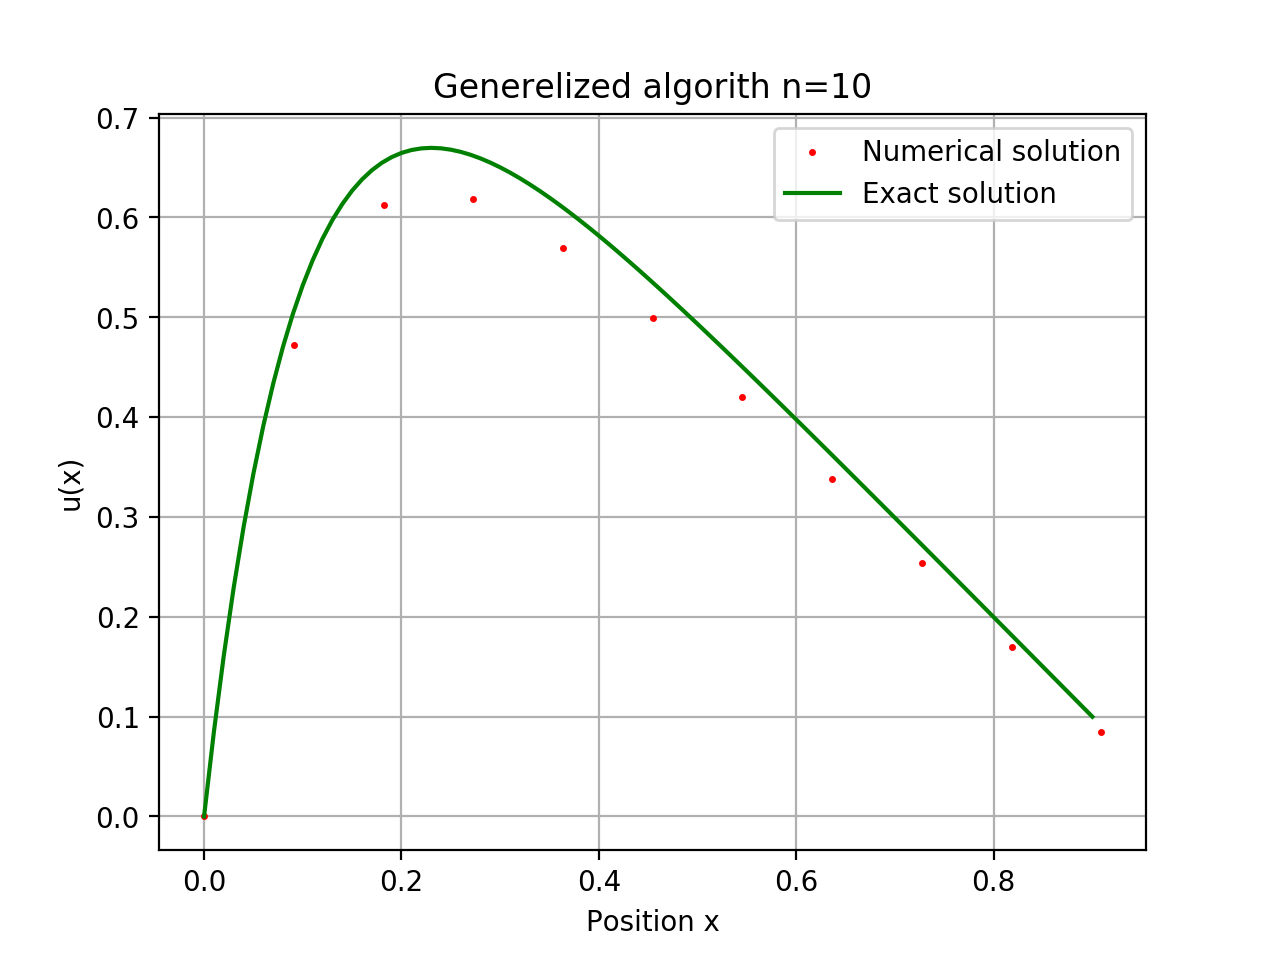
\includegraphics[scale=0.5]{alg-0-n10plot.png}
  \caption{General algorithm for n=10 plot points and the exact solution on the interval $x\in (0,1)$.}
  \label{fig:plotn10}
\end{figure}
\begin{figure}[H]
  \center
  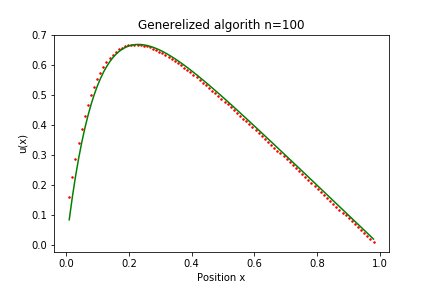
\includegraphics[scale=0.5]{alg-0-n100plot.png}  \caption{General algorithm for n=100 plot points and the exact solution on the interval $x\in (0,1)$.}
  \label{fig:plotn100}
\end{figure}
\begin{figure}[H]
  \center
  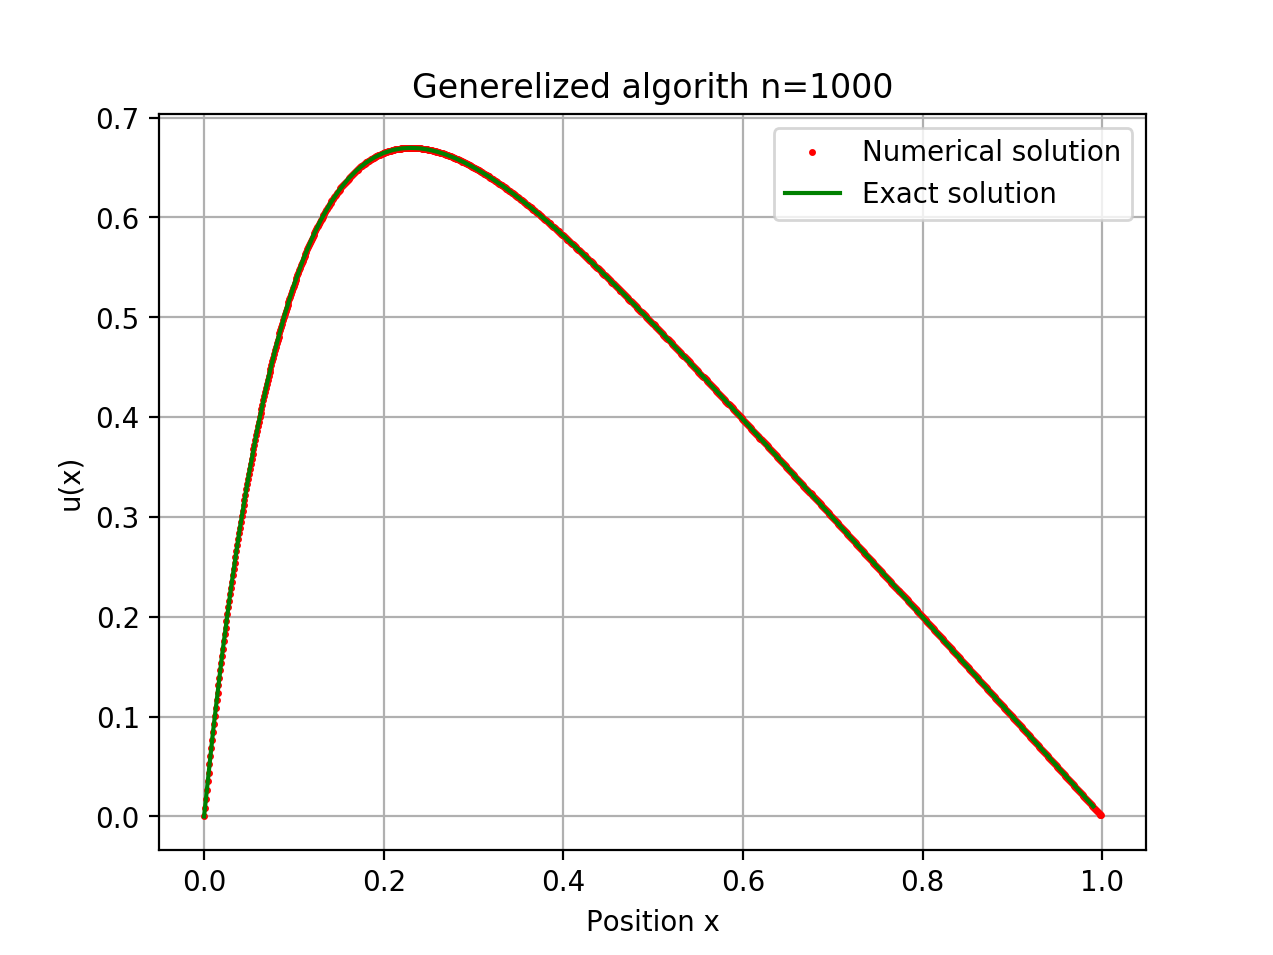
\includegraphics[scale=0.5]{alg-0-n1000plot.png}
  \caption{General algorithm for n=1000 plot points and the exact solution on the interval $x\in (0,1)$.}
  \label{fig:plotn1000}
\end{figure}

I see that for n=10, the difference between the exact solution and the numerical solution at the points $x_i=ih$ is big compared to the numerical solution when $n=100$ and $n=1000$. This is because the approximation uses the Taylor expansion of $u(x_i\pm h)$ and I supposes that the terms $h^2~0$, but for a step length of $h=\frac{1}{11}$. This means that $h^2$ is not small enough to suppose it is zero.

It is also worth noting that since I use a static step length, i.e. it is a fixed length, I do not care about the steepness of the slope, this can cause errors. I see that for $n=100$, the length between the plotted solution at $x_i$ when $x_i\in (0,0.2)$ is big, while when $x_i\in (0.2,1)$ the length between the plotted solution is small. A way to fix this is to take into account the first derivative of $u(x)$ and make the step length dependent on it.

By running the different algorithms 10 times for different numbers of gridpoints I get the following mean times.
\hfill\break

\captionof{table}{Mean time of the different algorithms run 10 times and their standard deviations (STD)}

\centering
\scalebox{0.8}{
    \begin{tabular}{||c|c|c|c||}
      \hline\hline 
      & \multicolumn{3}{|c||}{Mean time $\pm$ STD}\\
      \hline
  Number of gridpoints & General algorithm  & Specialized algorithm & LU decomposition \\
  \hline
  10 & $1,4\times 10^{-6}$ s $\pm 1\times 10^{-6}$ s& 
  $3,0\times 10^{-7}$ s $\pm 1 \times 10^{-7}$ s &  
  $6\times 10^{-4}$ s $\pm 2 \times 10^{-3}$ s \\
  \hline
  $10^2$ & $5,1\times 10^{-6}$ s $\pm 5 \times 10^{-7}$ s &
  $2,31\times 10^{-6}$ s $\pm 8 \times 10^{-8}$ s &
  $5\times 10^{-4}$ s $\pm 3\times 10^{-4}$ s \\
  \hline
  $10^3$ & $4,7 \times 10^{-5}$ s $\pm 4 \times 10^{-6}$ s &
  $2,27\times 10^{-5}$ s $\pm 3 \times 10^{-7}$ s &
  $3,8\times 10^{-2}$ s $\pm 4\times 10^{-3}$ s \\
  \hline
  $10^4$ & $4,4 \times 10^{-4}$ s $\pm 7 \times 10^{-5}$ s &
  $2,16\times 10^{-4}$ s $\pm 8 \times 10^{-6}$ s &
  $6$ s $\pm 1$ s \\
  \hline 
  $10^5$ & $4,4 \times 10^{-3}$ s $\pm 3 \times 10^{-4}$ s&
  $2,2\times 10^{-3}$ s $\pm 2 \times 10^{-4}$ s & N/A\\
  \hline
  $10^6$ &$2,4 \times 10^{-2}$ s $\pm 4 \times 10^{-3}$ s &
  $2,1\times 10^{-2}$ s $\pm 1 \times 10^{-3}$ s & N/A \\
  \hline\hline  
\end{tabular}
}

\hfill\break

I see the expected result that the specialized algorithm is faster for smaller $n$, this is because the number of FLOPS done by the specialized algorithm is half of the FLOPS the general algorithm does. I also see that the time difference becomes smaller as the number of gridpoints increases. This is because as the number of gridpoints increases I move from using fast memory, i.e. the CPU cache, over to using slow memory. When this is the case, the time it takes to write and read from memory will be the main factor of time usage, which means that the time difference should decrease.
\hfill\break

The LU decomposition which was done using the Armadillo library did also perform as expected. The general LU decomposition does $\frac{2}{3}n^3$ FLOPS, but I expect that Armadillo is optimized in such a way that it notices if the matrix used has certain symmetries, thus it might do less FLOPS. But I know that it has do reserve memory for the matrix and the vectors, hence it reserves memory for at least $n\times n$ doubles. This means $8 n\times n$ bytes of memory. This means it has to do a lot more FLOPS, which means it will perform slower. When $n=10^4$ it has to reserve at least $0,8$ GB of memory, for $n=10^5$ it would have to reserve 80 GB of memory. This is far more than any standard pc has and would crash the program or the pc.
\hfill\break

It is important to note that the time the program takes is highly environment dependent. The times given in this report is from a Microsoft Surface Pro running a Intel i5-7300U CPU at 2,60GHz. If it is done by a stronger or weaker system it will get better or worse times. The times are also dependent on what the operative system (OS) is doing. It is therefore important to make sure that the pc is in the same state when running the program.
\hfill\break

The relative error for the specialized algorithm is calculated using equation (\ref{eq:rel_error}) and is compared to the number of grid points in table (\ref{tb:error}). It is also plotted as a function of $\log{(n)}$ in figure (\ref{fig:rel_error}).


\begin{center}
  \captionof{table}{Maximum error of the specialized algorithm for n=10 to n=$10^7$.}\label{tb:error}
  \begin{tabular}{||c|c||}

    \hline\hline Number of gridpoints & Max relative error \\
    \hline
    10 & -1.2 \\
    \hline
    $10^2$ & -3.1 \\
    \hline
    $10^3$ & -5.1 \\ 
    \hline
    $10^4$ & -7.1 \\
    \hline
    $10^5$ & -9.1 \\ 
    \hline
    $10^6$ & -10.8\\
    \hline
    $10^7$ & -9.5\\
    \hline\hline
    
  \end{tabular}
\end{center}

\begin{figure}[H]
  \centering  
  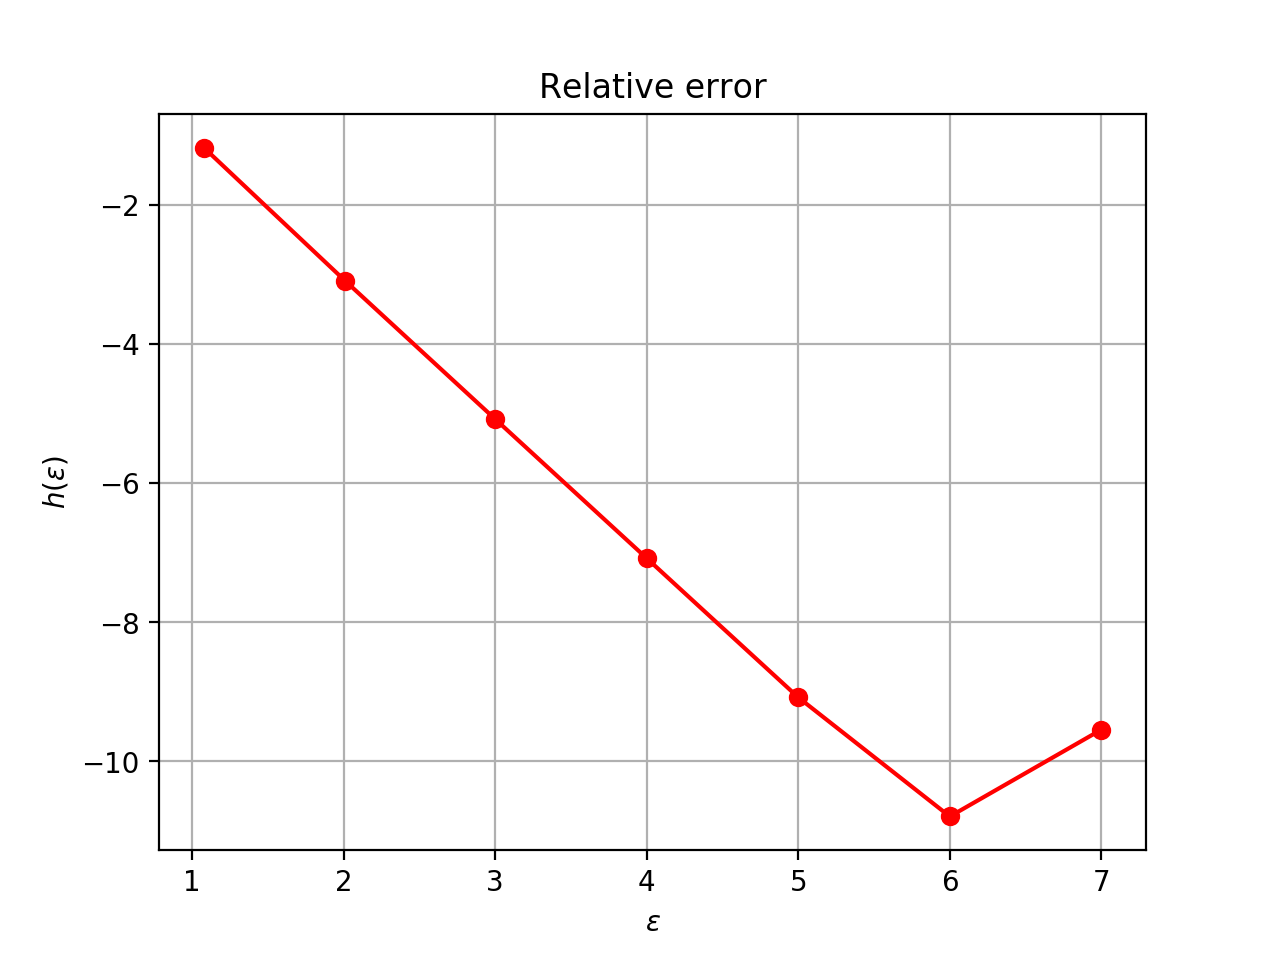
\includegraphics[scale=0.5]{relative_error.png}
  \caption{Plot of relative error as a function of $\log{(n)}$.}
  \label{fig:rel_error}
\end{figure}

I see that the relative error decreases linearly as a function of $\log{n}$  from $\log{(n)}=1 $ until $n=10^6$, when $n=10^7$ I see that the relative error increases. If there was no loss of precision I would expect $\epsilon$ to continue to decrease, but due to the fact that the computed expression has to take into account the machine error, this is not the case. 
\hfill\break

I see from the expression of the total error given by equation (\ref{eq:total_error}) that the error will decrease linearly when $n^2<<10^{15}$ but as $n^2$ becomes larger it will have more impact. From equation (\ref{eq:error_n}) I can plug in that $|u^{(4)}_0|=10^4$ which gives that the error is smallest when $n\approx1,2\times 10^{5}$. I can therefore see that the loss of numerical precision comes into play when $\log{(n)}\geq 5$ because of round off errors.

\section{Conclusions}
I found that optimizing an algorithm for a specific problem reduces the computation time and that choosing a general algorithm such as the LU decomposition to solve a simple problem is highly ineffective. The time a program uses is dependent on number of FLOPS it does and the number of memory read and write. If the number of memory read and write becomes big enough the computer has to use slow memory which means that the number of FLOPS does not matter as much. This was evident when comparing the mean time used by the general algorithm and the specialized algorithm. When the number of gridpoints were $n=10$, the specialized algorithm performed almost five times as fast as the general algorithm, since $t_{general}/t_{specialized}=(1,4\times 10^{-6}s/3,0\times10^{-7}s\approx 5)$, but when the number of grid points were $n=10^6$, the specialized and the general algorithm performed almost equal in time. I also found that the relative error decreases linearly as a function of $\log{(n)}$ until the round off error starts to dominate. The loss of precision became evident when the number of gridpoints exceeded $10^5$. This is because the machine error becomes dominating when $n> 1,2\times 10^{5}$. 

\printbibliography

\end{document}

